
% JuliaCon proceedings template
\documentclass{juliacon}
\setcounter{page}{1}

\usepackage{amsmath}
\usepackage{listings}

\begin{document}

% **************GENERATED FILE, DO NOT EDIT**************

\title{My JuliaCon proceeding}

\author[1]{1st author}
\author[1, 2]{2nd author}
\author[2]{3rd author}
\affil[1]{University}
\affil[2]{National Lab}

\keywords{Julia, Optimization, Game theory, Compiler}



\maketitle

\begin{abstract}
This work evaluates the feasibility of employing the Julia SciML ecosystem, the package NeuralPDE.jl in particular, to solve real-world problems, such as wildfire propagation prediction, using Physics-Informed Neural Networks. The aim is to re-implement some key parts of the widely used Weather Research and Forecasting WRF-SFIRE simulator by replacing its core differential equations numerical solvers with state-of-the-art physics-informed machine learning techniques to solve ODEs and PDEs, in order to transform it into a real-time simulator for wildfire spread prediction.
%\headingtable
\end{abstract}

\section{Introduction}
In recent years wildfires have been increasingly growing in intensity and frequency, becoming a serious threat to the health and socio-economic stability of various countries all over the world. In particular, Australia was devastated by the "Black Summer", the bushfire season between 2019 and 2020, and California just suffered from the most severe wildfire season recorded in its modern history. According to the California Department of Forestry and Fire Protection \cite{Gauk}: over 4 percent of its land was burned by more than 8,600 fires \cite{CALFIRE}.
In such a worrisome scenario, having the support of fast and accurate wildfire spread simulators that can run \textbf{iteratively} in order to evaluate several different containment strategies is of unprecedented importance.

\subsection{Real-time is revolutionary}
The current stable version of WRF is able to produce highly accurate and validated predictions, but each simulation takes several hours, which is acceptable for a single run. Nevertheless, if one wants to use the simulator for containment strategies, time is a major obstacle. In order to use WRF for that purpose, one should run the simulator iteratively with different initial scenarios, therefore predicting the outcome of various containment strategies and choosing the best one according to the output of the program. The revolutionary reach of such an approach is that it would limit human error in situations where taking the right decision quickly is extremely difficult. To reach this goal it is essential to significantly increase the computational efficiency of fire spread models, which can be done thanks to Machine Learning techniques.

\subsection{The need for SciML in this setting}
\textit{In the context of science, the well-known adage “a picture is worth a thousand words” might well be “a model is worth a thousand datasets.”}, writes Christopher Rackauckas in his trademark paper \cite{Rackauckas}. A single sentence couldn't describe the true power of Scientific Machine Learning better. Machine Learning's utmost strength, i.e. universal flexibility to approximate any nonlinearity from data, as stated by the Universal Approximation Theorem \cite{Kurkova}, is at the same time its main drawback: the higher the complexity of the problem, the more data the algorithm needs to train.
While some fields can provide big data, such as bioinformatics \cite{Yu}, many scientific disciplines are still limited in the use of Deep Learning (DL) by a lack of data. Another reason for the ineffectiveness of Machine Learning (ML) might be the apparent chaotic nature of a phenomenon. This is the case of wildfires and weather-related phenomena, which don't depend solely on the initial and boundary conditions, but evolve according to complex internal dynamics that cannot be predicted from mere data. In order to make a neural network learn such dynamics, one would need data with both high spatial and temporal resolution, something not available in this field \cite{Cenci}.
For this reason, we think that the growing field of Scientific Machine Learning is a good compromise where climate and wildfire science could take advantage. The idea is to embed physical information, generally in the form of partial differential equations, into the ML model, thus constructing a Physics Informed Neural Network (PINN). A data-driven physics-informed approach consists in training the model on data and constraining the solution space to the physically admissible ones (e.g. for incompressible fluid dynamics, any flow solution that breaks the mass conservation principle would not be considered by the model \cite{raissi}).
Another physics-informed architecture - the one considered in our case - consists instead in training the neural network directly on the governing equations of the physical phenomenon, employing the feed-forward networks as an efficient approximator of trajectories in the solution space. This approach leads to various advantages, such as avoiding the so-called \textit{curse of dimensionality}: as the dimensionality of an equation increases, the computational costs of a numerical equation solver grow exponentially, while PINNs can be proven to have a polynomial bound \cite{Grohs}. This results in a significant speed up with respect to numerical solvers when solving high dimensional problems.
We decided to use the second technique since our goal is to evaluate the feasibility of a high efficiency, ML-based, wildfire spread simulator that uses the equations of the WRF-SFIRE model.

\subsection{Why Julia?}
To develop our PINNs model, the natural choice for the language was Julia: its high perfomance together with a high level interface makes it easy to develop complex models in an easy yet performant manner. The ease of use is supported by the rich Scientific Machine Learning ecosystem and its community: packages like \textit{ModelingToolkit.jl} and \textit{NeuralPDE.jl} (\cite{zubov2021neuralpde}) have proved to be a valuable tool for scientific computation and dynamical systems analysis.
The usage of a high-level interface is a key advantage of the above-mentioned packages. This is crucial when the equations are complex and have a lot parameters. To get a sense of what that means, take a look at the following lines of code, which are much more intuitive compared to other languages:

\lstset{escapeinside=''}
\begin{lstlisting}[language = Julia]
using NeuralPDE, Flux, ModelingToolkit, GalacticOptim, 
Optim, DiffEqFlux

#Declarations
@parameters x y 
@variables u(..)
Dxx = Differential(x)^2
Dyy = Differential(y)^2

# Equation
eq = Dxx(u(x,y)) + Dyy(u(x,y)) ~ 
     sin(2π*x)*cos(2π*y)

# Boundary conditions
bcs = [u(0,y) '$\thicksim$' 0.f0, u(1,y) '$\thicksim$' -sin(pi*1)*sin(pi*y),
       u(x,0) '$\thicksim$' 0.f0, u(x,1) '$\thicksim$' -sin(pi*x)*sin(pi*1)]

# Domains
domains = [x '$\in$' IntervalDomain(0.0,1.0),
           y '$\in$' IntervalDomain(0.0,1.0)]

# Neural network
dim = 2  #number of dimensions
chain = Chain(Dense(dim,16,Flux.tanhshrink),
        Dense(16,16,Flux.tanhshrink),Dense(16,1))

# Discretization
dx, dy = 0.05, 0.05
strategy = NeuralPDE.GridTraining(0.1)
discretization = NeuralPDE.PhysicsInformedNN(chain, strategy)

cb = function (p,l)
    println("Current loss is: $l")
    return false
end

# Problem statement and solution
pde_system = PDESystem(eq,bcs,domains,[x,y],[u])
prob = discretize(pde_system,discretization)

res = GalacticOptim.solve(prob, ADAM(0.05); cb = cb,
      maxiters=500)
phi = discretization.phi

xs,ys = 0.0 : dx : 1.0, 0.0 : dy : 1.0

u_predict = reshape([first(phi([x,y],res.minimizer))
            for x in xs for y in ys],(length(xs),length(ys)))
\end{lstlisting}


\section{The new architecture}
Firstly, we started by investigating the structure of the systems of partial differential equations (PDEs) that constitute the core of the physical model of WRF-SFIRE. In this way we detected the modules where replacing the current structure has the greatest impact (i.e. CPU overhead). As expected, numerical solvers of the model's main differential equations are responsible for more than $20\%$ of the total overhead. In particular, the level set equation (a PDE which describes the spread of the fireline, according to the level set method) and the Euler system (a system of 7 PDEs governing the atmosphere behavior), have significant impacts on the CPU load during fire simulation. We will describe them in detail in the next paragraph.
\textbf{Therefore, we will present a detailed application of the PINN architecture to the level set equation and we will outline some ideas about the implementation of Euler system.} \\

\begin{figure}[t]
\centering
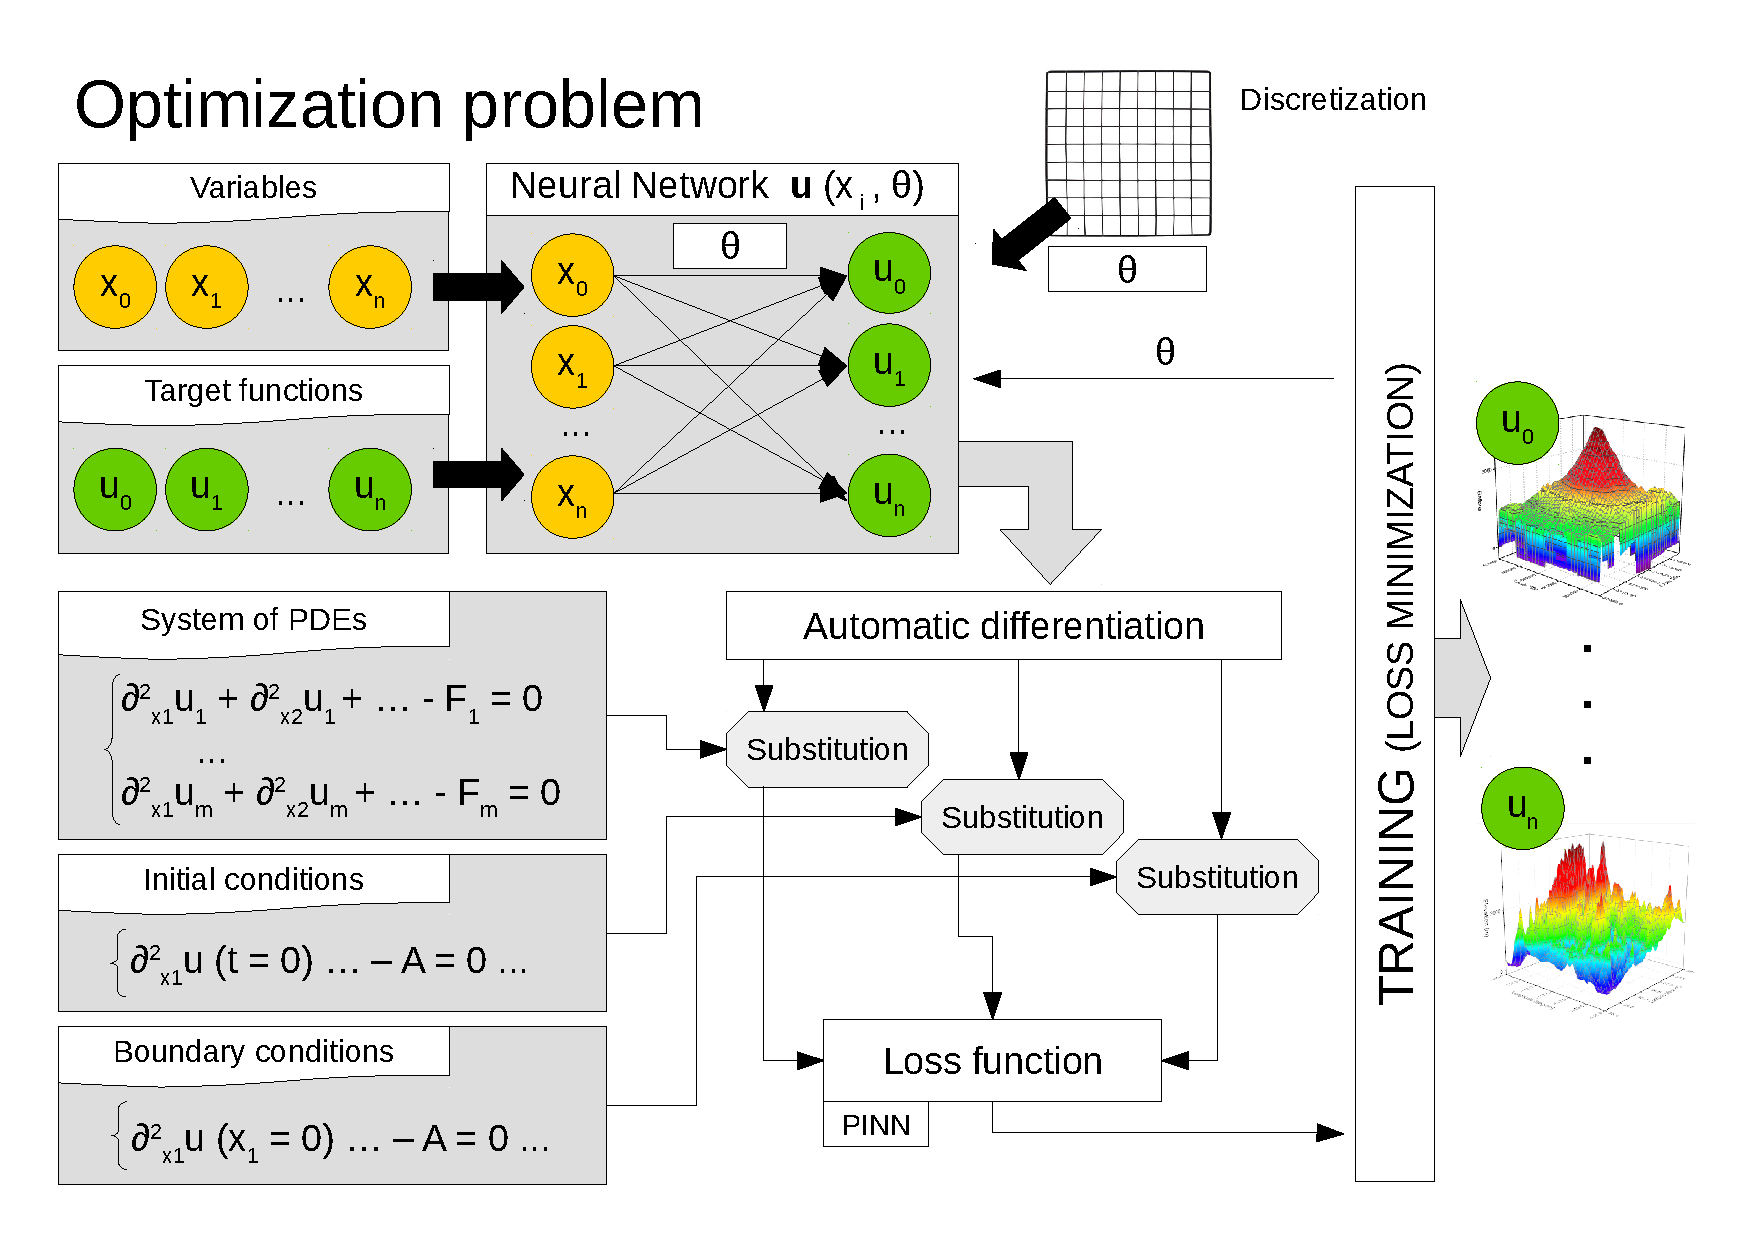
\includegraphics[width=0.518\textwidth]{images/Optimization problem.pdf}
\caption{Physics-informed neural network architecture for solving PDEs}
\label{fig:forcesneural}
\end{figure}

Let's now delve into the structure of this architecture. We have replaced the original numerical solvers with a profoundly different approach, by taking advantage of the recently developed Julia packages \textit{NeuralPDE.jl} and \textit{DiffEqFlux.jl} \cite{DiffEqFlux.jl}, which support Physics Informed Neural Networks (PINNs) for automated PDE solving and Backwards Stochastic Differential Equation (BSDE) methods to deal with parabolic PDEs.
We employed the former method: PINNs are feed forward neural networks that are trained to solve supervised learning tasks while respecting any given law of physics described by general nonlinear partial differential equations. The resulting neural networks form a new class of universal function approximators that naturally encode any underlying physical laws as prior information \cite{zubov}.

The underlying architecture can be summarized by the following steps, with reference to Fig.\ref{fig:forcesneural}. Let's put ourselves in the most general case, where we want to find \textit{n} target functions $[u_1,...,u_n]$ which satisfy a system of \textit{n} PDEs. We first construct a surrogate solution to \textit{u(x)} as a neural network \textit{\^{u}(x;$\theta$)} with \textit{m} inputs (where \textit{m} is the number of independent variables), \textit{n} outputs and parameters $\theta$; since a neural network is mathematically a composite function, the derivatives of \textit{\^{u}} with respect to its input can be evaluated by applying the chain rule for differentiating compositions of functions using automatic differentiation (AD). Then we need to define a loss function (we used the $L^2$ norm) in order to calculate the discrepancy between $[u_1,...,u_n]$ and the outputs of the neural network: this is where we force our network to satisfy the physics imposed by the PDEs. Indeed, the loss is defined by substituting our neural network and its derivatives back into the equations we want to solve (where we brought all the terms on the left-hand side of the equal sign). The last step is to train the neural network to find the best parameters by minimizing the loss function with gradient-based optimizers, such as Adam or LBFGS. It is straightforward that minimizing the loss function means solving the equations, since we are approximating our target functions with \textit{\^{u}} better and better. \textbf{The key point is that it converts an integration problem into a minimization task and it does not need data to train, because it is trained on the PDEs themselves}. 


\section{Mathematical structure} 
\paragraph{Atmospheric governing equations}
The flux form conserved prognostic variables are defined as
\begin{equation} \label{prognostic variables}
    \begin{cases}
    \textbf{V} = \mu_d\textbf{v} = (U,V,W) \\
    \Omega = \mu_d\omega \\
    \Theta_m = \mu_d\theta_m \\
    Q_m = \mu_dq_m \\
    \end{cases}
\end{equation}
where $\mu_d = \partial_\eta p_d$ is the vertical coordinate metric, $\textbf{v} = (u,v,w)$ are the covariant velocities in the horizontal and vertical directions, $\omega = \dot{\eta}$ is the contravariant vertical velocity, $ \theta_m $ is the moist potential temperature and $q_m = q_v,q_c,q_r...$ denote the mixing ratios of moisture variables.
Accordingly, the flux-form Euler equations, representing the core of the ARW, can be written as follows \cite{ARW-WRF}:
\vspace{1mm}

\noindent{\textit{Conservation of momentum}}
\begin{equation}
\begin{cases}
\partial_t U + (\nabla \cdot Vu) + \mu_d\alpha\partial_x p + (\frac{\alpha}{\alpha_d})\partial_\eta p\partial_x \phi = F_U \\
\partial_t V + (\nabla \cdot Vv) + \mu_d\alpha\partial_y p + (\frac{\alpha}{\alpha_d})\partial_\eta p\partial_y \phi = F_V \\
\partial_t W + (\nabla \cdot Vw) - g[(\frac{\alpha}{\alpha_d})\partial_\eta p - \mu_d]= F_w \\
\end{cases}
\label{eqn:Momentum}
\end{equation}
\textit{Conservation of heat}
\begin{equation}
    \partial_t \Theta_m + (\nabla \cdot V\theta_m) = F_{\Theta_m}
    \label{eqn:Energy}
\end{equation}
\textit{Conservation of mass}
\begin{equation}
    \partial_t\mu_d + (\nabla \cdot V) = 0
\label{eqn:Mass}
\end{equation}
\textit{Geopotential Material Derivative}
\begin{equation}
    \partial_t\phi + \mu_d^{-1} [(V \cdot \nabla\phi) - gW] = 0
    \label{eqn:geopotential}
\end{equation}
\textit{Scalar moisture equations}
\begin{equation}
    \partial_t Q_m + (\nabla \cdot Vq_m) = F_{Q_m}
    \label{eqn:moisture}
\end{equation}
where $$\nabla \cdot Va= \partial_x(Ua) + \partial_y (Va) + \partial_\eta (\Omega a)$$ and $$V \cdot \nabla a= U\partial_xa + V\partial_ya + \Omega\partial_\eta a,$$ for a generic variable $a$.  

These equations are coupled with the \textit{diagnostic equation for dry hydrostatic pressure}
\begin{equation}
    \partial_{\eta} \phi = -\alpha_d\mu_d 
    \label{eqn:diagdry}
\end{equation}
and the \textit{ diagnostic relation for the full pressure} (dry air combined with water vapor)
\begin{equation}
    p=p_0 \Big (\frac{R_d\theta_m}{p_0\alpha_d}\Big)^{\gamma} 
\end{equation}

In Eq. \eqref{eqn:Momentum} - \eqref{eqn:moisture}, $\alpha_d = \frac{1}{p_d}$ is the inverse density of dry air, $\alpha= \alpha_d (1+q_v + q_c + q_r +...)^{-1}$, while $R_d$ is the gas constant for dry hair and $\gamma= \frac{c_p}{c_v}=1.4$ is the ratio of the heat capacities for dry air. The right hand side terms $F_U, F_V, F_W, F_{\Theta_m}$ contain the Coriolis and curvature terms along with mixing terms and physical forcings. 

\paragraph{Level set equation}
In SFIRE \cite{Mandel}, the propagation of a fire burning in the area $\Sigma=\Sigma(t)$ in the horizontal $(x,y)$ plane on which the Earth is projected, is implemented by the level set method, which evolves a function $\psi = \psi(x,t)$, called the \textit{level set function}, such that the burning area at a time $t$ is $$ \Sigma(t) = \{ x: \psi(x,t)\leq0\}$$ and the fireline $\Gamma(t)$, i.e. the boundary of the burning region $\Sigma(t)$, is the level set 
\begin{equation}\label{fireline}
  \Gamma(t)= \{ x: \psi(x,t)=0\}.  
\end{equation}

The evolution of the level set function is governed by the partial differential equation 
\begin{equation}\label{level set}
   \partial_t \psi + S ||\nabla \psi || = 0,
\end{equation}
called the \textit{level set equation}.
The model adopts a semi-empirical approach, where the fire spread rate $S$ is computed from fuel properties, using the following modified Rothermel formula \cite{rothermel}: 
\begin{equation}\label{Rothermel}
    S= R_0 (1+ \phi_W + \phi_S).
\end{equation}
Here, $R_0$ represents the spread rate in the absence of wind, whereas $\phi_W$ and $\phi_S$ are respectively the wind factor and the slope factor. 
In WRF, this equation is solved numerically through discretization on the refined fire grid, adopting Heun's method, a second-order Runge Kutta method (\cite{Mandel}, p.596). 


\section{Implementation of the Level set}
The level-set differential equation is, as previously explained, the mathematical core for calculating the spread of the fire. The level set equation (that is a 2D surface embedded in a 3D euclidean space) is initially set as the distance of each point from the ignition's line. Our approach requires that every quantity is provided either as a constant or as a function. Therefore we implemented the initial condition as a cone with elliptical section, because we had to deal with circular and linear ignition shapes (theoretically, any ignition shape can be given as input). The cone is then shifted down in order to make the contour level $z = 0$ resembling the desired initial fire line (see the Appendix for a graphical representation). Multiple ignition points are possible, but further refinements are needed to make this possibility fully functional.
The algorithm contains all the necessary expressions for the calculation of the fire spread rate, taking into account the values of the wind, the altimetric profile, the fuel map etc. These variables have to be given in input as differentiable vector fields of space and time.
This can be considered both a limit and an advantage, in fact on one hand the discretized measurements must be fitted using approximating functions, but on the other hand this method is computationally efficient. The possibility to give in input finite matrix of values is presented in "Future Work" and depends on the fact that some key libraries we use are still under development.
You can see in the appendix an example of the altimetric profile of the \textit{Isom Creek} fire location fitted using a 4th degree polynomial. 
The last step before the training of the model is a proportional scaling of the values to a domain with size in the order of $10^{1}$ and the definition of a discretization that is used only to run the training algorithm. The outputs will be continuous functions. The discretization to this interval prevents some numerical instabilities and spikes that are linked to the early stage of development of some Julia libraries in use. The loss function is made of two parts: the former minimizing the $L^2$ error referred to the PDE definition and the latter minimizing the $L^2$ distance between the boundary conditions and the solution evaluated at the boundaries. At this point the training algorithm is instantiated and launched. The minimization of the loss function is the process that actually solves the PDE and constitutes the main load for the CPU. It can be easily parallelized and thus accelerated using GPUs.
When the training is completed the prediction undergoes a new proportional scaling that gives back the original domain shape.


\subsection{Ideal simulation: "One fire"}
For clarity, we renamed the \textit{Two Fires} ideal simulation as \textit{One Fire}, after having removed one ignition point. It is a simple case that demonstrates that our model works well on the level set in case of fires that spread in flat areas where the fuel doesn't change. It also evolves according to the wind direction, represented by a vector with two components. The results at different time frames are represented in Fig.\ref{fig:one_fire_sequence}.
The details about the architecture employed and the training are listed in TABLE \ref{table:specs_one_fire}.


\begin{table}
\tbl{Technical Specs of the model - Domain sizes are expressed in arbitrary units, since scaling factors transform input and output in pre-processing and post-processing phases.}{
\label{table:specs_one_fire}
\begin{tabular}{  l  p{3.0cm}  }\hline
\textbf{Optimization Algorithm}      
& ADAM (4800 iterations)
\\\hline

\textbf{Final Objective Value}
& 6.39 e-8
\\\hline
 
\textbf{Training Strategy}
& QuadratureTraining()  
\\\hline
 
\textbf{Domains}
& $t\in[0,10]$, $x\in[0,10]$, $y\in[0,10]$
\\\hline
  
\textbf{Training Mesh Size}
& $[dt,dx,dy] = [0.17,0.02,0.02]$
\\\hline
 
\textbf{Initial Condition}
& $\psi(0,x,y) = (5 (x - 0.3)^2 + 0.15 y^2)^{\frac{1}{2}} - 0.2$ 
\\\hline

\textbf{Neural Network dimensions}
& $3>16>1$
\\\hline

\textbf{Training Time}
& 647 s
\\\hline
\end{tabular}}
\end{table}



\begin{figure}[t]
\centering
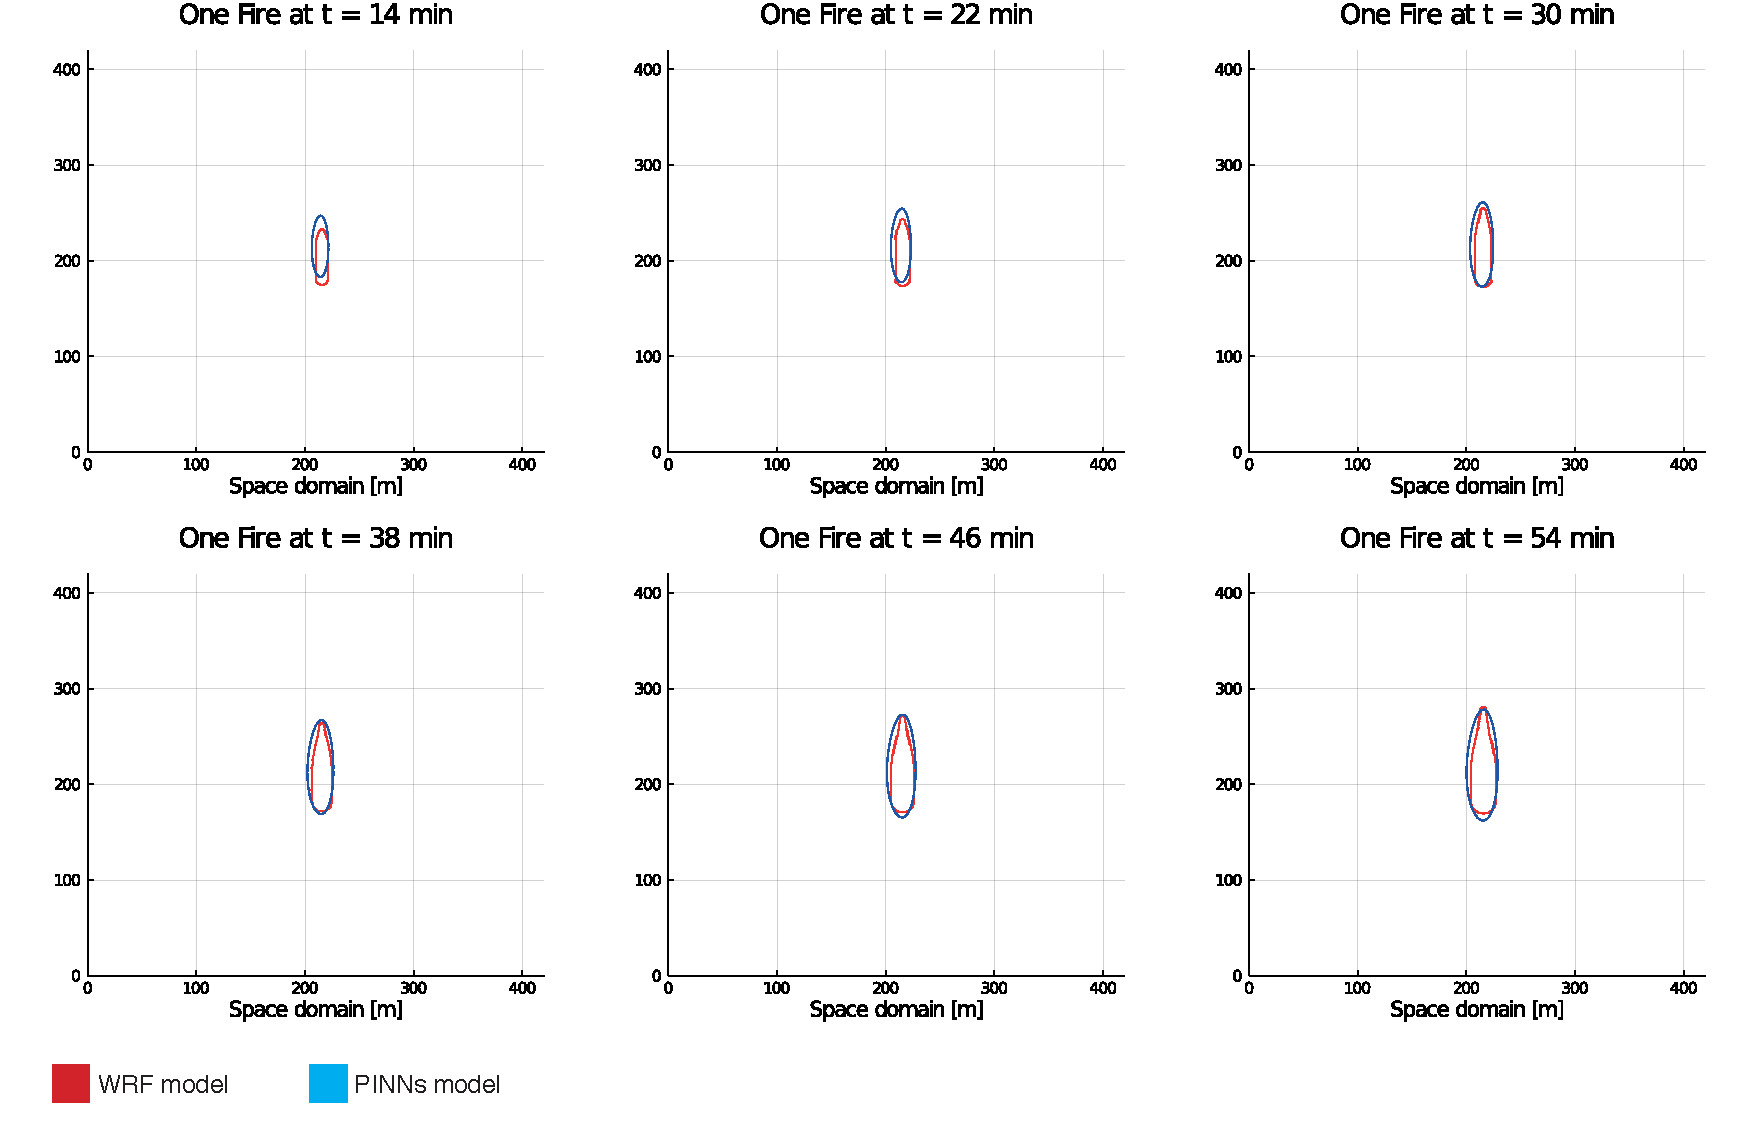
\includegraphics[width=0.45\textwidth]{images/one_fire_results/One Fire sequence.pdf}
\caption{Comparison between the WRF and PINNs outputs at different time frames}
\label{fig:one_fire_sequence}
\end{figure}

In order to provide a quantitative measure of the error between the outputs we decided to use the Hausdorff distance \cite{Knauer},
\begin{displaymath}
    d_{\mathrm H}(X,Y) = \max\left\{\,\sup_{x \in X} \inf_{y \in Y} d(x,y),\, \sup_{y \in Y} \inf_{x \in X} d(x,y)\,\right\},
\end{displaymath}
normalized on the area of the curves that represent the fireline, as Fig.\ref{fig:hausdorff_one_fire} shows. The fact that the error decreases tells us that as the area grows with time, the difference between the two regions doesn't increase, meaning that they evolve in synchrony and with the same shape.


\begin{figure}[t]
\centering
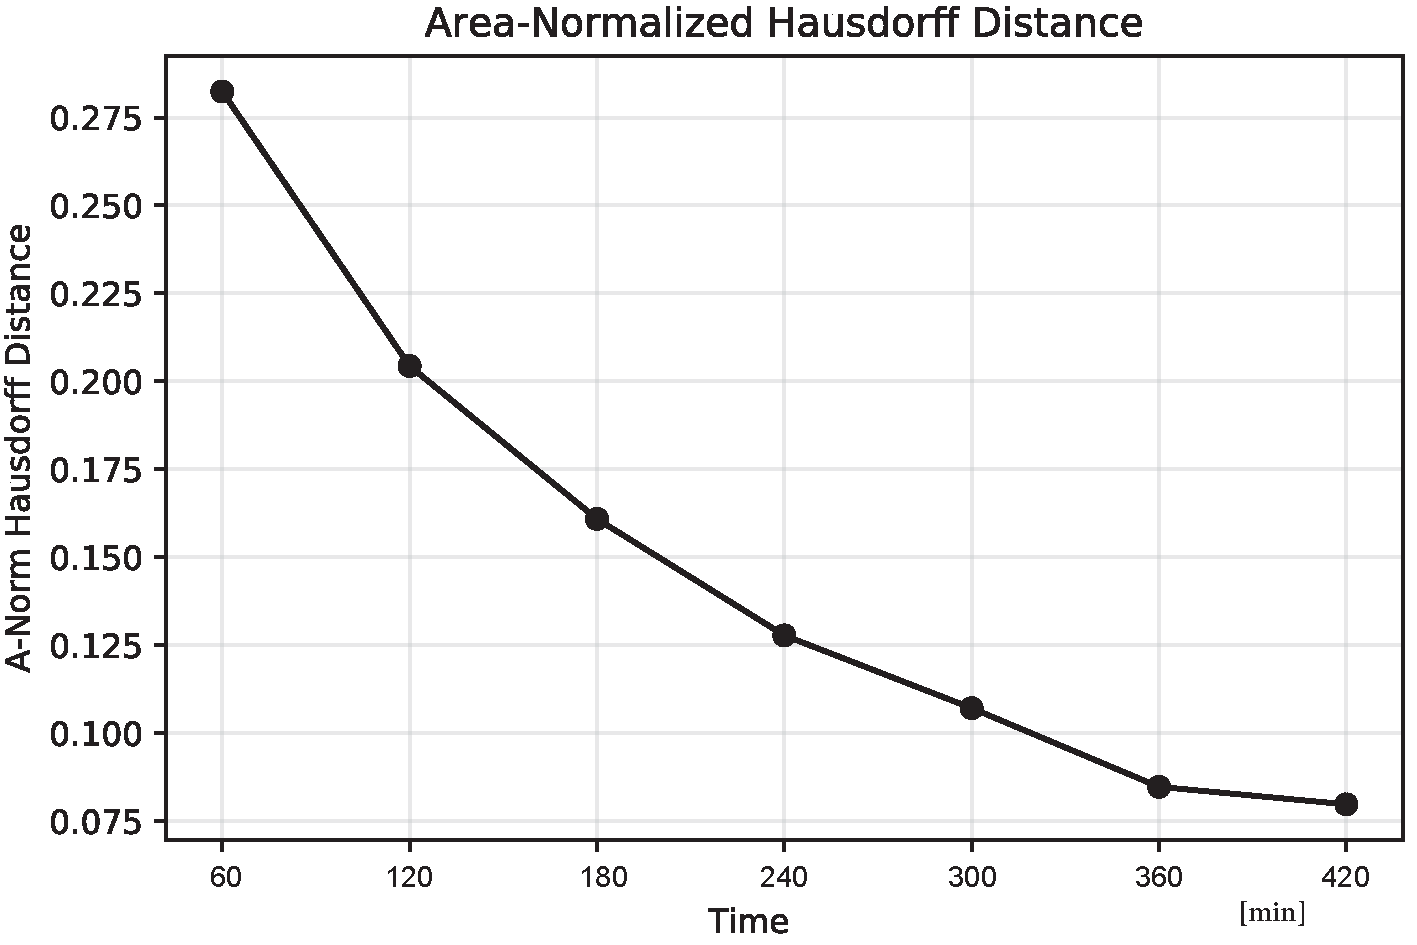
\includegraphics[width=0.4\textwidth]{images/Hausdorff/norm_area_hausdorff_one_fire2.pdf}
\caption{Hausdorff distance as a measure of the error - One Fire.}
\label{fig:hausdorff_one_fire}
\end{figure}


\subsection{Simulation of a real wildfire: Isom Creek, Alaska, 6/5/2020}

We have been able to simulate the Isom Creek fire \cite{isom_creek_info} both with WRF and with our implementation. Although it is not possible to perform a precise quantitative comparison between WRF and the real data, or between our result and the real data (due to a lack of temporal precision of the available data at \cite{isom_creek_map}, it is clear that the WRF output simulates the wildfire accurately, at least visually.
The result obtained with the PINN architecture is shown in Fig.\ref{fig:isom_sequence}.
It is clear that our implementation hasn't been able to capture the shape of the fireline with the same accuracy. This will be pointed out below as a temporary limitation to our model: at the moment it is not possible to assign a different fuel category to each mesh point (i.e. using a matrix to build a function), so the fireline will always have a smooth perimeter.
The specifics of the architecture are outlined in TABLE \ref{table:isom_specs}.

\vspace{2pt}


\begin{table}
\tbl{Technical Specs of the model - The considerations on measurement units made in TABLE 1 apply also here.}{
\label{table:isom_specs}
\begin{tabular}{  l  p{3.0cm}  }\hline
\textbf{Optimization Algorithm}      
& ADAM (3000 iterations) 
\\\hline
 
\textbf{Final Objective Value}
& 2.14 e-6
\\\hline
 
\textbf{Training Strategy}
& QuadratureTraining()  
\\\hline
 
\textbf{Domains}
& $t\in[0,10] $, $x\in[0,10] $, $y\in[0,10]$
\\\hline
  
\textbf{Training Mesh Size}
& $[dt,dx,dy] = [0.17, 0.02, 0.02]$  
\\\hline
 
\textbf{Initial Condition}
& $\psi(0,x,y)=((x-5)^2 + 0.7 (y-5)^2)^{\frac{1}{2}}-0.2$
\\\hline

\textbf{Neural Network dimensions}
& $3>16>1$
\\\hline

\textbf{Training Time}
& 270 s
\\\hline
\end{tabular}}
\end{table}


\begin{figure}[t]
\centering
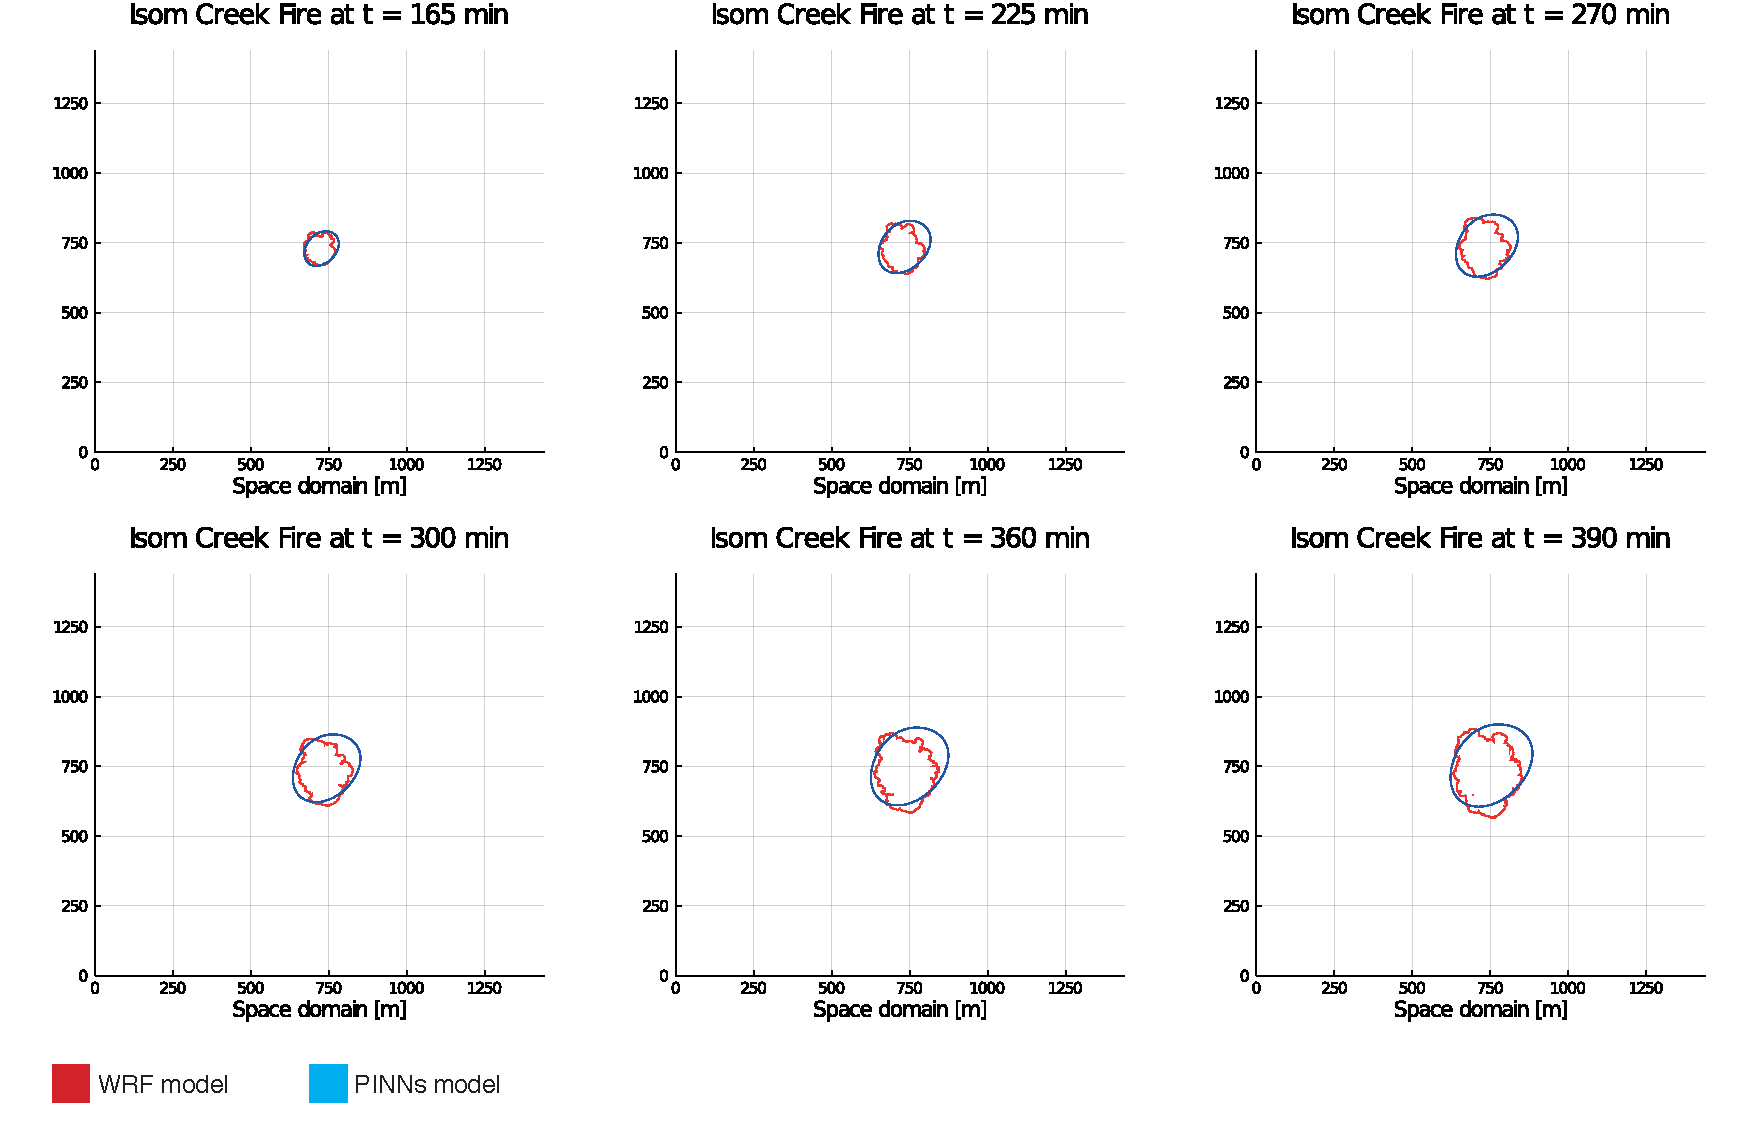
\includegraphics[width=0.45\textwidth]{images/isom_creek_results/Isom creek sequencepdf.pdf}
\caption{Comparison between the WRF and PINNs outputs at different time frames}
\label{fig:isom_sequence}
\end{figure}

The error can be quantitatively measured with the Hausdorff distance as before, with the outcome plotted in Fig.\ref{fig:hausdorff_isom}.  

\begin{figure}[t]
\centering
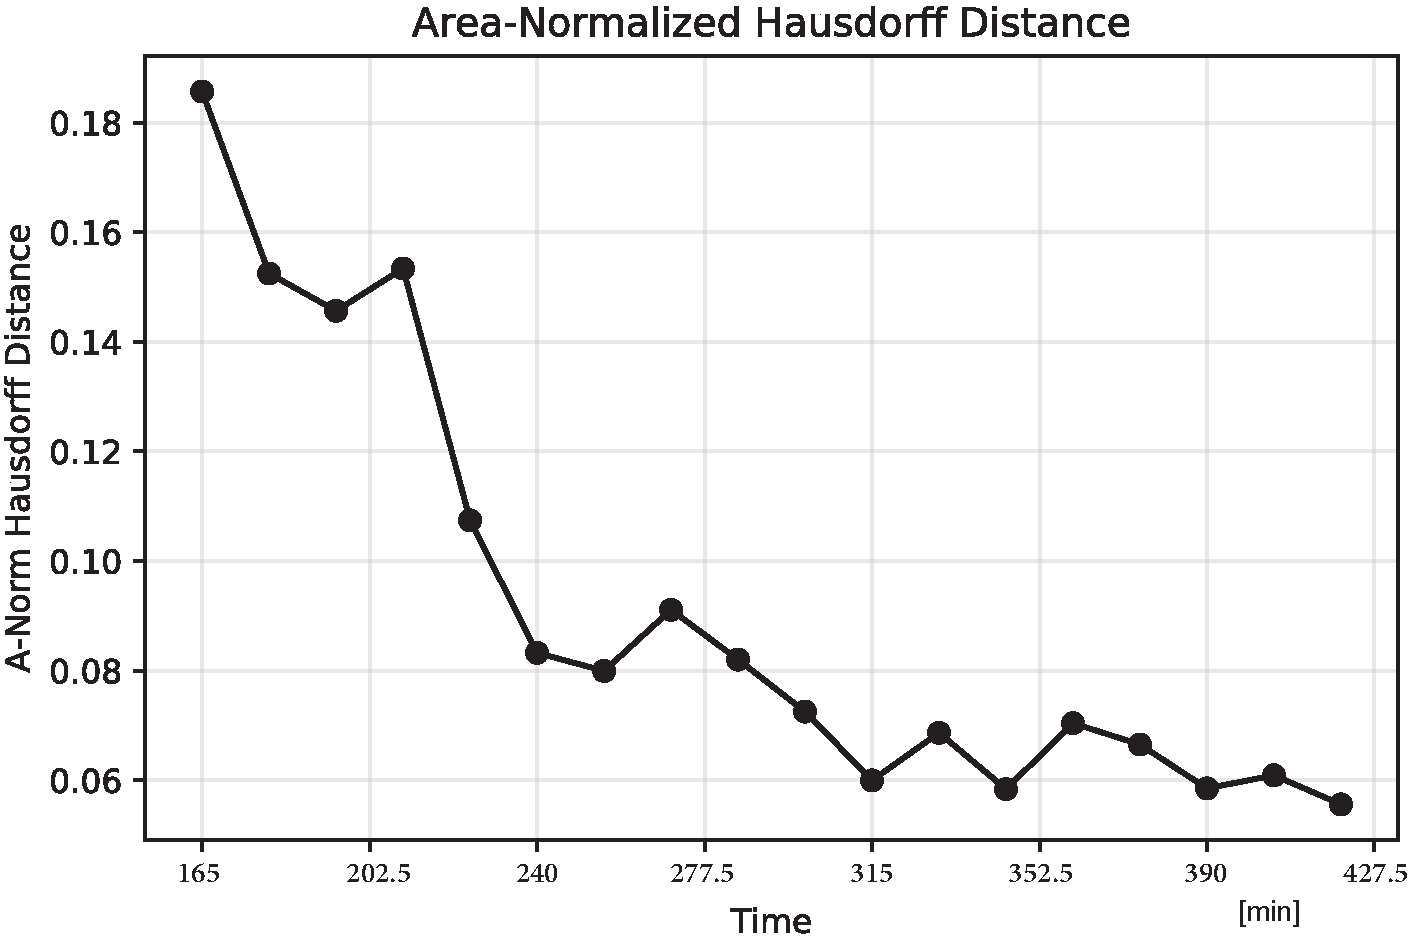
\includegraphics[width=0.4\textwidth]{images/Hausdorff/norm_area_ISOM2.pdf}
\caption{Hausdorff distance as a measure of the error - Isom Creek.}
\label{fig:hausdorff_isom}
\end{figure}

The considerations outlined in the previous paragraph remain valid here.

\section{Discussion}\label{discussion}

\subsection{Implementation of the Euler system}
On top of the results previously outlined, we have also taken on the implementation of the most computationally expensive part of the WRF physical model. Writing and solving the 7-equation Euler system in Julia was really challenging, in fact at the moment we are not aware of any publications where these techniques are yet applied to PDE systems of such complexity. The first problem was to figure out which were the independent and dependent variables: climate models adopt different conventions depending on the circumstances (e.g. they generally use pressure coordinates instead of height coordinates).
Then we had to choose the most suitable training strategy, which turned out to be \textit{QuadratureTraining}. We have used parabolic initial conditions for a first evaluation, but we want to investigate them more in depth, since the study of boundary conditions often deserves a paper on its own. Unfortunately, the \textit{NeuralPDE} library is still unable to treat this kind of problem with stability, and often incurs errors due to internal divergence calculations. Despite this, we have been able to obtain convergence of the loss function, although it is not enough to present valid results.
The results exposed above show the feasibility of utilizing the Julia \textit{NeuralPDE.jl} library to model a wildfire related differential equation, i.e. the level set equation. As disclosed above, we have also obtained some preliminary but unstable results regarding the atmospheric coupling of the model by attempting to solve the Flux-Form Euler system equation.
The outputs obtained with our approach don't strictly follow the jagged firelines of WRF: that's not an intrinsic limit of the architecture, which doesn't lack variance even if it is rather simple; the reason is, as explained above, that the inputs (fuel and wind in particular) we gave to the NN are not varied enough, due to limitations of the library.
In spite of this we have shown the ability of our implementation to reproduce the desired time evolution of the fireline as given by WRF.


\subsection{Advantages of this architecture}\label{advantages}
The various advantages of this approach are:

\begin{itemize}
    \itemsep0em 
    \item We can get a rough estimate of the speed up our model provides - compared to numerical solvers - by noting that the training time is of some hundreds of seconds, while the WRF run time is more than an hour. This point has to be further studied: on one hand, we used a simpler set of inputs for the reasons we will explain later; on the other hand we worked on one of the eight cores at our disposal.
    \item While numerical methods only solve on the initial domain range, this architecture learns the neural network parameters that can be used to \textbf{extend the predicted solution outside of the training domains} (with a decrease in accuracy if the extrapolation is extended too much). This can be used for "forensic investigations": it is possible to reconstruct the ignition point and the evolution of the fireline from the final state of the wildfire.
    \item It is possible to interpolate the solution on a continuous mesh.
    \item Modifying the equations of the model is as easy as changing a few lines of code, instead of re-implementing the discretization and perturbative form of the equations, allowing for faster investigation of new models. However, the \textit{NeuralPDE.jl} package provides low-level interfaces for users seeking more personalised implementations.
    \item Given the possibility to use several CPU cores and GPU acceleration, the speed could increase even more and this approach could be run iteratively in order to simulate the outcome of different \textit{containment scenarios} and choose the best among them.
    \item This architecture doesn't need neural networks with a high number of degrees of freedom to be accurate, reducing the overall computational cost and increasing performance. In quantitative terms, this means not exceeding some tens of neurons on a single hidden layer. 
    \item As a consequence, the model is more interpretable (it is less similar to a complete \textit{black-box}) and its users can run the resulting simulator on standard PCs without needing high performance machines.
    \item PINNs can be used to extrapolate physical laws once they have been interpolated, hence providing a tool to refine theoretical models. However, this requires a greater amount of input data.
\end{itemize}

\subsection{Limitations}\label{limitations}
Let's now analyze the limits of our approach:

\begin{itemize}
    \itemsep0em
    \item At the moment, it cannot run on GPUs nor multiple CPUs because the library we used is not fully developed yet. We contacted the developers and they are working on it.
    \item The library doesn't support the usage of matrices as functions of their indices. This means it is not possible to use a variable fuel map, fundamental in order to capture the evolution of the fire with higher accuracy. We opened an issue about this \cite{issue177}.
    \item Our approach suffers from numerical instability depending on the training strategy adopted and on the number of neurons and layers.
    \item The model only works on relatively small domains and is unstable for larger ones. Since the output has a small codomain, we had to scale the quantities involved up and introduce a scale factor on the fire spread rate in order to make it compatible with the evolution of the output of WRF.
    \item We still have to figure out how to predict the spread of a wildfire with more than one ignition point.
    \item The architecture has not yet been extended to Convolutional Neural Networks, Recurrent Neural Networks or others.
    \item The exceptions thrown by low level code are often difficult to debug due to the early stage of develpment of some libraries.
    \item The direct conversion of a PINNs problem to a numerical one (ODEProblem) for \textit{DifferentialEquation.jl} is possible only in special cases.
\end{itemize}

\section{Future work}
This research is the first step towards a concrete implementation of PINNs-based wildfire simulation. We have designed a chart (Fig.\ref{fig:future_work}) that shows the next improvements to be made in order to achieve such an ambitious goal.

\begin{figure}[t]
\centering
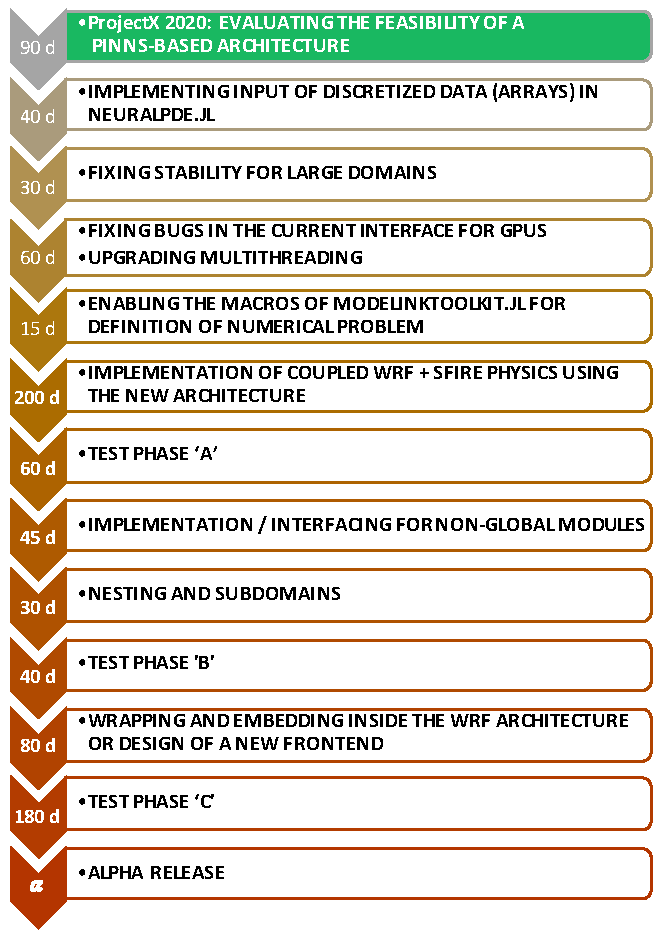
\includegraphics[width=0.4\textwidth]{images/future_work.pdf}
\caption{Future prospect of our work}
\label{fig:future_work}
\end{figure}

\section{Conclusions}
The study we carried out had the goal to investigate the applicability of the recently developed field of Scientific Machine Learning on climate, wildfires in particular, models, using the programming language Julia. We have outlined some results that tell us that many improvements are needed in order to transform this into a validated product, but also show the big potential of our approach. We need to add further refinements to the implementation in order to carry out a precise time comparison between the two approaches, but the results obtained thus far show promising evidence.
The encouraging outcome inspires us to continue our work by improving the architectures and possibly employ them in different fields of research.
We hope that this work will be part of a line of research devoted to a more effective cohesiveness between Machine Learning and Physical Models, and thus further explored by other researchers.

\section{Acknowledgments}
This work was presented at the ProjectX 2020 competition by UofT AI.
We acknowledge University of Turin, Machine Learning Journal Club for supporting.
We thank Professor Enrico Ferrero (Università del Piemonte Orientale), Professor Massimiliano Manfrin (University of Turin) and the whole Atmospheric Physics and Metereology Group, PhD Christopher Rackauckas (Massachussets Institute of Technology), PhD Kirill Zubov (Saint-Petesburg State University), Vaibhav Dixit (Julia Computing), PhD Brian Wee (Founder at Massive Connections), Dr. Rustem Arif Albayrak (NASA), PhD David Marvin (CEO at Salo Sciences), Professor Piero Fariselli (University of Turin) and Pietro Monticone M.Sc. student (University of Turin), for their precious help and availability.
We acknowledge the company \textit{Mollificio Astigiano} (Belveglio, Asti, Italy) for providing the computational power needed for this research and the\textit{HPC4AI} center of the University of Turin for their support.

% **************GENERATED FILE, DO NOT EDIT**************

\bibliographystyle{juliacon}
\bibliography{ref.bib}


\clearpage

\section{Appendix}
All the code produced is published on a public repository available at this link:\\ https://github.com/MachineLearningJournalClub/MLJC-UniTo-ProjectX-2020-public.
The output of the WRF simulations can be found in the following Google Drive folder: %\\  https://drive.google.com/drive/folders/1wUCKUyVwC0Pf-e9WlLiqOxRLF0or2D0U?usp=sharing\\ or 
https://tinyurl.com/mljc-unito-px2020.
\vspace{10pt}

\begin{figure}[h]
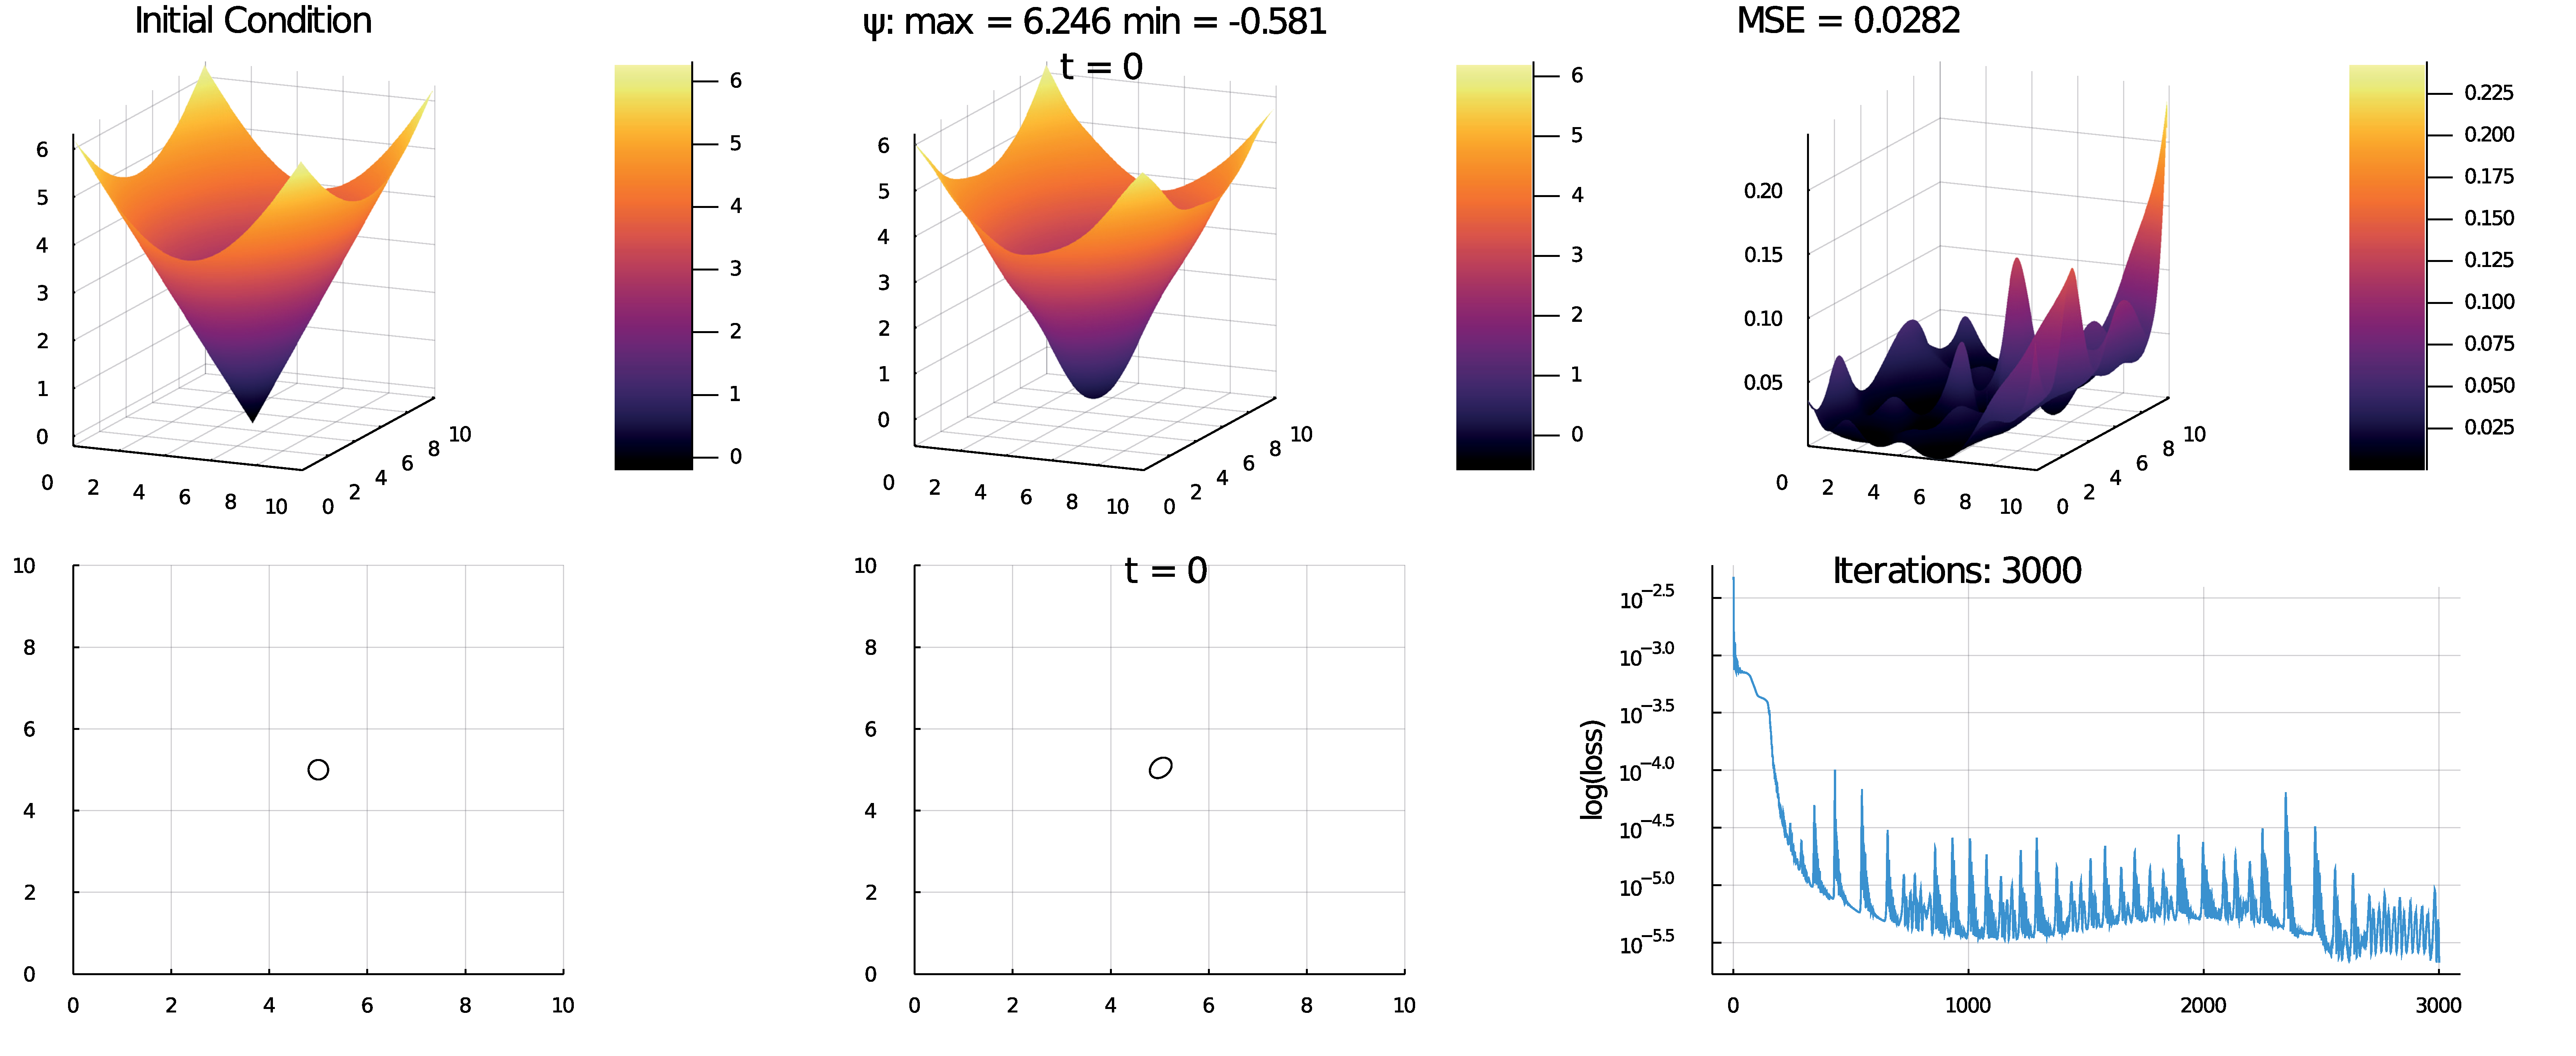
\includegraphics[width=1\textwidth]{images/BC_Isom.pdf}
\caption{Boundary condition comparison and training - Isom Creek}
\end{figure}

\begin{figure}[h]
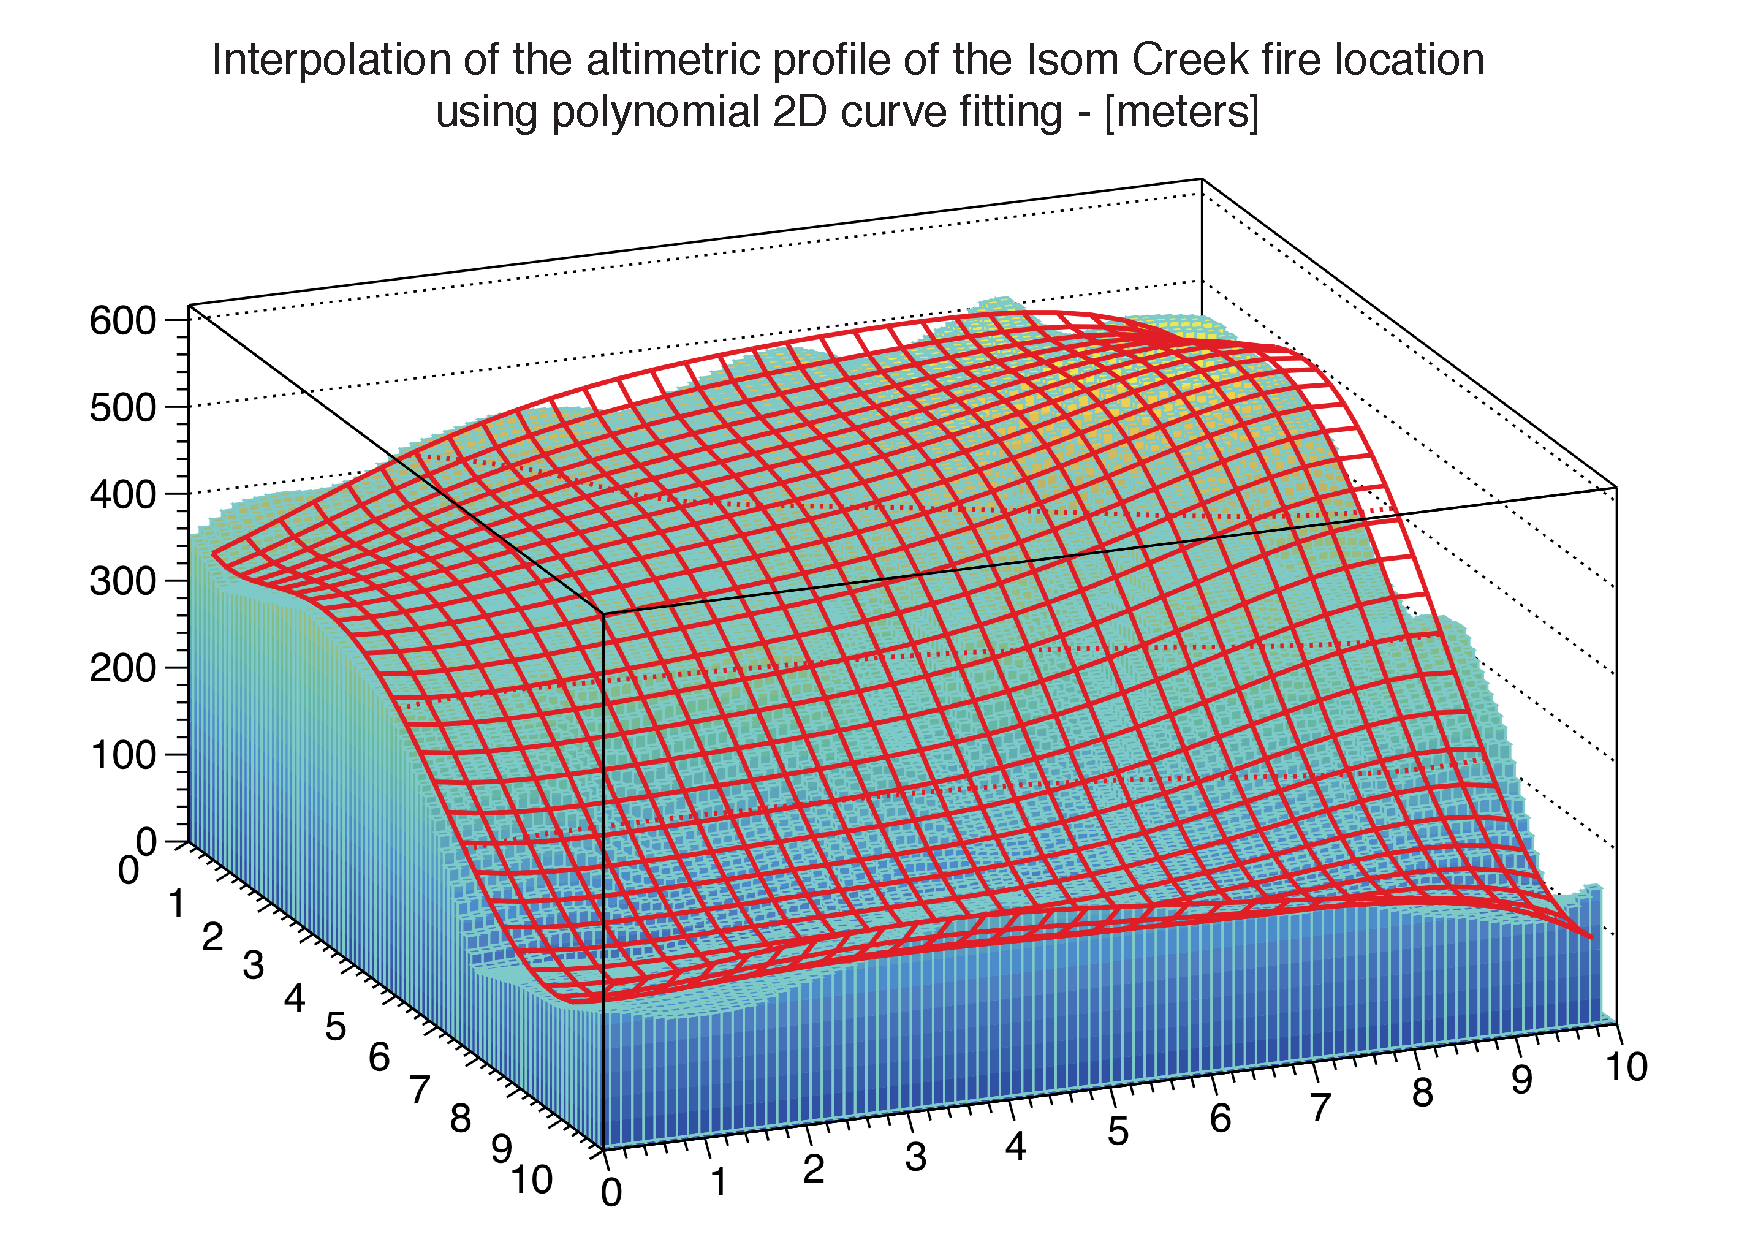
\includegraphics[width=0.5\textwidth]{images/interpolation.pdf}
\caption{Altimetric profile interpolation of the Isom Creek fire region.}
\end{figure}

\end{document}

% Inspired by the International Journal of Computer Applications template
